%%% LaTeX Template: Article/Thesis/etc. with colored headings and special fonts
%%%
%%% Source: http://www.howtotex.com/
%%% Feel free to distribute this template, but please keep to referal to http://www.howtotex.com/ here.
%%% February 2011
%%%
%%% Modified January 2016 by CDM

%%%  Preamble
\documentclass[11pt,letterpaper]{article}
\usepackage[margin=1.0in]{geometry}
\usepackage[T1]{fontenc}
\usepackage[bitstream-charter]{mathdesign}
\usepackage[latin1]{inputenc}					
\usepackage{amsmath}						
\usepackage{xcolor}
\usepackage{cite}
\usepackage{hyphenat}
\usepackage{graphicx}
\usepackage{float}
\usepackage{subfigure}
\usepackage{sectsty}
\usepackage[compact]{titlesec} 
\usepackage[tablegrid]{vhistory}
\usepackage{pbox}
\allsectionsfont{\color{accentcolor}\scshape\selectfont}

%%% Definitions
\definecolor{accentcolor}{rgb}{0.0,0.0,0.5} 
\newcommand{\teamname}{Team Hawt Wheels}
\newcommand{\productname}{Smart Cart}
\newcommand{\coursename}{CSE 4316: Senior Design I}
\newcommand{\semester}{Spring 2016}
\newcommand{\docname}{Architectural Design Specification}
\newcommand{\department}{Department of Computer Science \& Engineering}
\newcommand{\university}{The University of Texas at Arlington}
\newcommand{\authors}{David Harvey \\ Dennis Otieno \\ Peggy Soh \\ Brian Wong \\ Or Zoarets}

%%% Headers and footers
\usepackage{fancyhdr}
	\pagestyle{fancy}						% Enabling the custom headers/footers
\usepackage{lastpage}	
	% Header (empty)
	\lhead{}
	\chead{}
	\rhead{}
	% Footer
	\lfoot{\footnotesize \teamname \ - \semester}
	\cfoot{}
	\rfoot{\footnotesize page \thepage\ of \pageref{LastPage}}	% "Page 1 of 2"
	\renewcommand{\headrulewidth}{0.0pt}
	\renewcommand{\footrulewidth}{0.4pt}

%%% Change the abstract environment
\usepackage[runin]{abstract}			% runin option for a run-in title
%\setlength\absleftindent{30pt}			% left margin
%\setlength\absrightindent{30pt}		% right margin
\abslabeldelim{\quad}	
\setlength{\abstitleskip}{-10pt}
\renewcommand{\abstractname}{}
\renewcommand{\abstracttextfont}{\color{accentcolor} \small \slshape}	% slanted text

%%% Start of the document
\begin{document}

%%% Cover sheet
{\centering \huge \color{accentcolor} \sc \textbf{\department \\ \university} \par}
\vspace{1 in}
{\centering \huge \color{accentcolor} \sc \textbf{\docname \\ \coursename \\ \semester} \par}
\vspace{0.5 in}
\begin{figure}[h!]
	\centering
   	
\includegraphics[width=0.60\textwidth]{images/smart_cart}
\end{figure}
\vspace{0.5 in}
{\centering \huge \color{accentcolor} \sc \textbf{\teamname \\ \productname} \par}
\vspace{0.5 in}
{\centering \large \sc \textbf{\authors} \par}
\newpage


%\vspace{1 in}
%\centerline{January 13th, 2012}
%\newpage

%%% Revision History
\begin{versionhistory}
  	\vhEntry{0.1}{03.11.2016}{DH, DO, PS, BW, OZ}{document creation}
  	\vhEntry{0.2}{04.08.2016}{DH, DO, PS, BW, OZ}{complete draft}
\end{versionhistory}
\newpage

%%% Table of contents
\setcounter{tocdepth}{2}
\tableofcontents
\newpage

%%% List of figures and tables (optional)
\listoffigures
\listoftables
\newpage

%%% Document sections
\section{Introduction}
\subsection{Product Concept}
The Smart Cart will provide assistance by being an autonomous carrier. The cart needs to be able to do the following things:
\begin{itemize}
	\item Follow a ''master'' to the designated destination
	\item Avoid collision with obstacles such as walls and other people
	\item Include an integrated power supply
	\item Holonomic mobility
\end{itemize}

\subsection{Scope}
The main function of the Smart Cart is to help its user carry tools from one point to another. It will also have an integrated power supply to allow its user to charge or power his or her tools. A unique feature of the Smart Cart is that the cart will identify and follow its "master" by using the Intel RealSense. Another unique feature of the cart is its holonomic wheels. This allows the cart to easily maneuver and avoid collisions with objects by using image processing from a camera. The Smart Cart will require external input from the user. The user must wear a colored band that is provided with the Smart Cart. This band is used by the cart for tracking its "master". External outputs produced by the cart will be messages to let its user know whether it has succesfully identified its master. There are no other external inputs or outputs. A simple user interface may be implemented for identification of master depending on the availability of time. 

\subsection{Key Requirements}
The Smart Cart shall have five layers that work in unison to allow the cart to autonomously navigate and follow a specified user. The five layers in the system are the Smart Cart layer, Power Supply layer, Imaging/Navigation layer and Crab Drive layer. The five layers will be discussed more in the following sections.
\newpage
\section{System Overview}
This section should describe the overall structure of your software system. Think of it as the strategy for how you will build the system. An architectural "layer" is the top-level logical view, or an abstraction, of your design. Layers should be composed of related elements of similar capabilities, and should be highly independent of other layers, but should have very clearly defined interfaces and interactions with other layers. Each layer should be identified individually and should be unique as to its function and purpose within the system. This section should also contain the high-level block diagram of the layers, as shown in the example below, as well as detailed descriptions of the functions of each layer.

\begin{figure}[h!]
	\centering
 	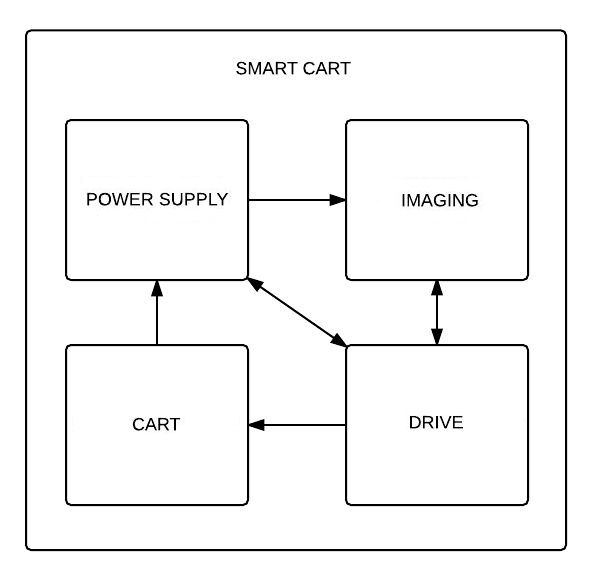
\includegraphics[width=0.60\textwidth]{images/system_overview}
 \caption{A simple architectural layer diagram}
\end{figure}


\subsection{Power Supply Layer Description}
Each layer should be described separately in detail. Descriptions should include the features, functions, critical interfaces and interactions of the layer. The description should clearly define the services that the layer provides. Also include any conventions that your team will use in describing the structure: naming conventions for layers, subsystems, modules, and data flows; interface specifications; how layers and subsystems are defined; etc.

\subsection{Cart Layer Description}
Each layer should be described separately in detail. Descriptions should include the features, functions, critical interfaces and interactions of the layer. The description should clearly define the services that the layer provides. Also include any conventions that your team will use in describing the structure: naming conventions for layers, subsystems, modules, and data flows; interface specifications; how layers and subsystems are defined; etc.

\subsection{Crab Drive Layer Description}
Each layer should be described separately in detail. Descriptions should include the features, functions, critical interfaces and interactions of the layer. The description should clearly define the services that the layer provides. Also include any conventions that your team will use in describing the structure: naming conventions for layers, subsystems, modules, and data flows; interface specifications; how layers and subsystems are defined; etc. 

\subsection{Imaging and Navigation Description}
Each layer should be described separately in detail. Descriptions should include the features, functions, critical interfaces and interactions of the layer. The description should clearly define the services that the layer provides. Also include any conventions that your team will use in describing the structure: naming conventions for layers, subsystems, modules, and data flows; interface specifications; how layers and subsystems are defined; etc. 
\newpage
\section{Subsystem Definitions \& Data Flow}
This section breaks down the simple architectural layer diagram with another level of detail. The logical subsystems that compose each layer and its interactions and interfaces between the subsystems are graphically represented. Even though the power supply layer does not have data flow, it is still a key layer to the system. The following data flow block diagram shows a high level diagram of all the layers in the Smart Cart.

\begin{figure}[h!]
	\centering
 	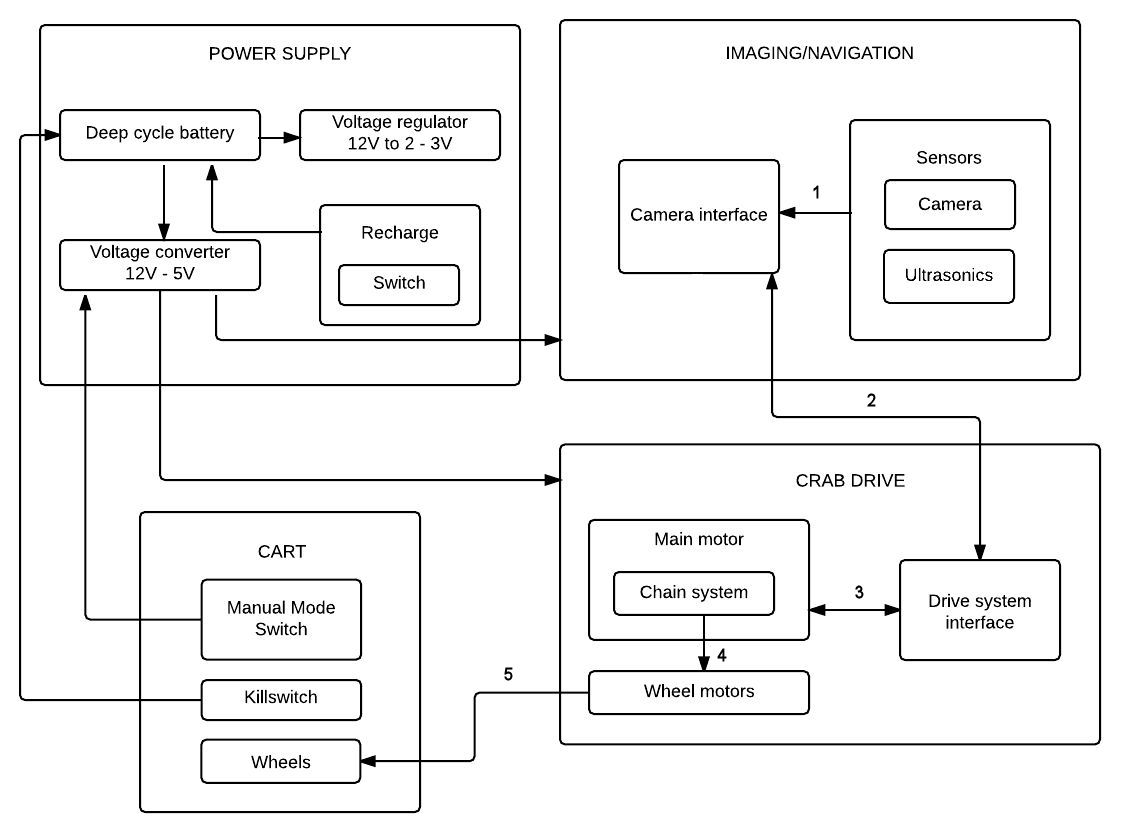
\includegraphics[width=\textwidth]{images/diagram_whole}
 \caption{A simple data flow diagram}
\end{figure}

\newpage
\section{X Layer Subsystems}
In this section, the layer is described in some detail in terms of its specific subsystems. Describe each of the layers and its subsystems in a separate chapter/major subsection of this document. The content of each subsystem description should be similar. Include in this section any special considerations and/or trade-offs considered for the approach you have chosen.

\subsection{Subsystem 1}
This section should be a general description of a particular subsystem for the given layer. For most subsystems, an extract of the architectural block diagram with data flows is useful. This should consist of the subsystem being described and those subsystems with which it communicates.

\begin{figure}[h!]
	\centering
 	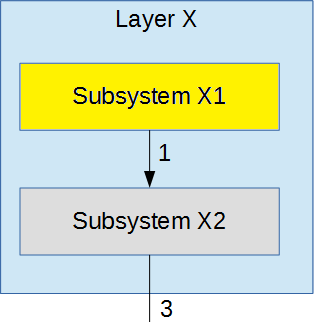
\includegraphics[width=0.60\textwidth]{images/subsystem}
 \caption{Example subsystem description diagram}
\end{figure}

\subsubsection{Assumptions}
Any assumptions made in the definition of the subsystem should be listed and described. Pay particular attention to assumptions concerning interfaces and interactions with other layers.

\subsubsection{Responsibilities}
Each of the responsibilities/features/functions/services of the subsystem as identified in the architectural summary must be expanded to more detailed responsibilities. These responsibilities form the basis for the identification of the finer-grained responsibilities of the layer's internal subsystems. Clearly describe what each subsystem does.

\subsubsection{Subsystem Interfaces}
Each of the inputs and outputs for the subsystem are defined here. Create a table with an entry for each labelled interface that connects to this subsystem. For each entry, describe any incoming and outgoing data elements will pass through this interface.

\begin {table}[H]
\caption {Subsystem interfaces} 
\begin{center}
    \begin{tabular}{ | p{1cm} | p{6cm} | p{3cm} | p{3cm} |}
    \hline
    ID & Description & Inputs & Outputs \\ \hline
    \#xx & Description of the interface/bus & \pbox{3cm}{input 1 \\ input 2} & \pbox{3cm}{output 1}  \\ \hline
    \#xx & Description of the interface/bus & \pbox{3cm}{N/A} & \pbox{3cm}{output 1}  \\ \hline
    \end{tabular}
\end{center}
\end{table}

\subsection{Subsystem 2}
Repeat for each subsystem

\subsection{Subsystem 3}
Repeat for each subsystem


\newpage
\section{Y Layer Subsystems}
In this section, the layer is described in some detail in terms of its specific subsystems. Describe each of the layers and its subsystems in a separate chapter/major subsection of this document. The content of each subsystem description should be similar. Include in this section any special considerations and/or trade-offs considered for the approach you have chosen.

\subsection{Subsystem 1}
This section should be a general description of a particular subsystem for the given layer. For most subsystems, an extract of the architectural block diagram with data flows is useful. This should consist of the subsystem being described and those subsystems with which it communicates.

\begin{figure}[h!]
	\centering
 	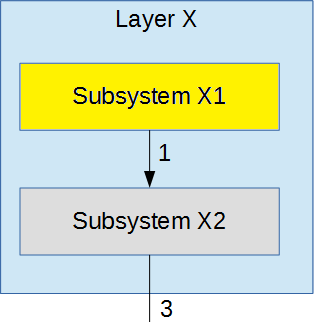
\includegraphics[width=0.60\textwidth]{images/subsystem}
 \caption{Example subsystem description diagram}
\end{figure}

\subsubsection{Assumptions}
Any assumptions made in the definition of the subsystem should be listed and described. Pay particular attention to assumptions concerning interfaces and interactions with other layers.

\subsubsection{Responsibilities}
Each of the responsibilities/features/functions/services of the subsystem as identified in the architectural summary must be expanded to more detailed responsibilities. These responsibilities form the basis for the identification of the finer-grained responsibilities of the layer's internal subsystems. Clearly describe what each subsystem does.

\subsubsection{Subsystem Interfaces}
Each of the inputs and outputs for the subsystem are defined here. Create a table with an entry for each labelled interface that connects to this subsystem. For each entry, describe any incoming and outgoing data elements will pass through this interface.

\begin {table}[H]
\caption {Subsystem interfaces} 
\begin{center}
    \begin{tabular}{ | p{1cm} | p{6cm} | p{3cm} | p{3cm} |}
    \hline
    ID & Description & Inputs & Outputs \\ \hline
    \#xx & Description of the interface/bus & \pbox{3cm}{input 1 \\ input 2} & \pbox{3cm}{output 1}  \\ \hline
    \#xx & Description of the interface/bus & \pbox{3cm}{N/A} & \pbox{3cm}{output 1}  \\ \hline
    \end{tabular}
\end{center}
\end{table}

\subsection{Subsystem 2}
Repeat for each subsystem

\subsection{Subsystem 3}
Repeat for each subsystem


\newpage
\section{Z Layer Subsystems}
In this section, the layer is described in some detail in terms of its specific subsystems. Describe each of the layers and its subsystems in a separate chapter/major subsection of this document. The content of each subsystem description should be similar. Include in this section any special considerations and/or trade-offs considered for the approach you have chosen.

\subsection{Subsystem 1}
This section should be a general description of a particular subsystem for the given layer. For most subsystems, an extract of the architectural block diagram with data flows is useful. This should consist of the subsystem being described and those subsystems with which it communicates.

\begin{figure}[h!]
	\centering
 	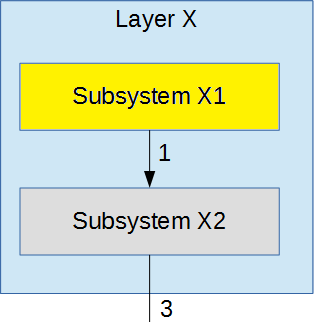
\includegraphics[width=0.60\textwidth]{images/subsystem}
 \caption{Example subsystem description diagram}
\end{figure}

\subsubsection{Assumptions}
Any assumptions made in the definition of the subsystem should be listed and described. Pay particular attention to assumptions concerning interfaces and interactions with other layers.

\subsubsection{Responsibilities}
Each of the responsibilities/features/functions/services of the subsystem as identified in the architectural summary must be expanded to more detailed responsibilities. These responsibilities form the basis for the identification of the finer-grained responsibilities of the layer's internal subsystems. Clearly describe what each subsystem does.

\subsubsection{Subsystem Interfaces}
Each of the inputs and outputs for the subsystem are defined here. Create a table with an entry for each labelled interface that connects to this subsystem. For each entry, describe any incoming and outgoing data elements will pass through this interface.

\begin {table}[H]
\caption {Subsystem interfaces} 
\begin{center}
    \begin{tabular}{ | p{1cm} | p{6cm} | p{3cm} | p{3cm} |}
    \hline
    ID & Description & Inputs & Outputs \\ \hline
    \#xx & Description of the interface/bus & \pbox{3cm}{input 1 \\ input 2} & \pbox{3cm}{output 1}  \\ \hline
    \#xx & Description of the interface/bus & \pbox{3cm}{N/A} & \pbox{3cm}{output 1}  \\ \hline
    \end{tabular}
\end{center}
\end{table}

\subsection{Subsystem 2}
Repeat for each subsystem

\subsection{Subsystem 3}
Repeat for each subsystem


\newpage

%%% References
\bibliographystyle{plain}
\bibliographystyle{reference/IEEEtran_custom}
\bibliography{reference/refs}{}

\end{document}